\section{Maps Merger}
This is not properly a side project, since it is, has it is, a completely uncorrelated project.
It has been placed altogheter with this project because, looking at the possible future developments, there will be the needing of merging two maps.

For our purposes, a map is a set of landmarks, where each landmark is defined by a couple of values (its \textbf{x} and \textbf{y} coordinates).
The assumption made is that the two maps overlap in some part, and we want to find out which is the transformation needed to overlap them. Once this is found, a global map can be extracted from the two.

The program uses the RANSAC algorithm to find the ``best'' transformation.
A model is identified from two couples of landmarks, each couple from one of the maps. In fact with the first correspondance we detect the translation, and with the second correspondance we detect the rotation.
For each of these models we count the overlapping landmarks amongst the whole sets and give a ``score'' to the model. The chosen model will be the one with the highest score.

Another useful assumption is that the two maps have approximatively the same scale, so when we analyze a model, if the distance between the two landmarks in the first map is very different from the distance between the landmarks in the second map, we can skip that model without the need of additional examinations. This usually reduces the number of possible models by some orders of magnitude.

\begin{figure}[htbp]
  \centering
    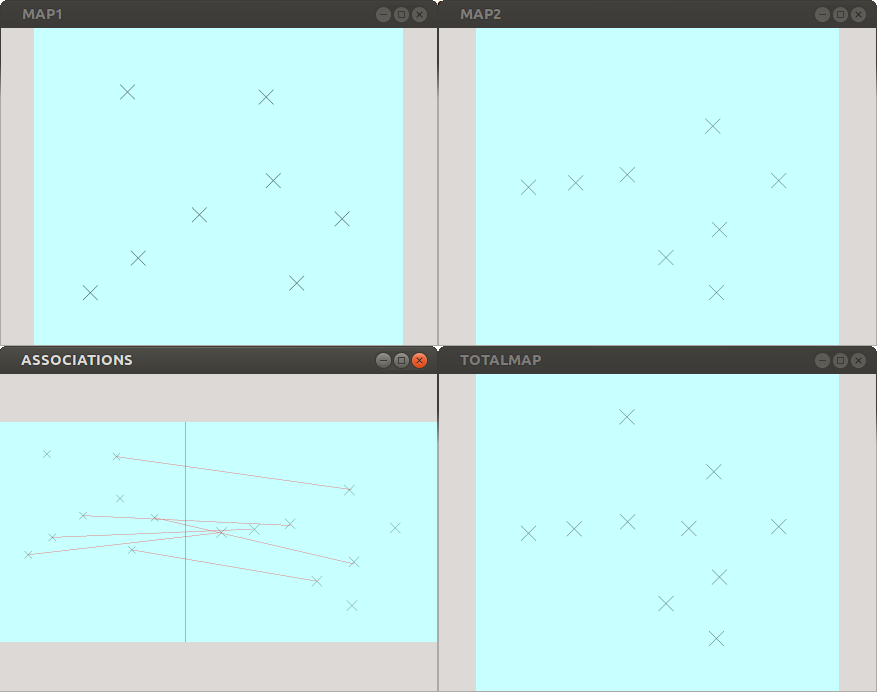
\includegraphics[width=0.8\textwidth]{images/mapsmerger.png}
  \caption{Screenshot of the MapsMerger program. In addition to rotation and translation, in the second map the landmarks have also been ``moved'' a little}
  \label{fig:mapsmerger}
\end{figure}
